\section*{Описание экспериментальной установки}

Схема экспериментальной установки для исследования дифракции Френеля на щели приведена на рисунке:

\begin{figure}[H]
	\centering
	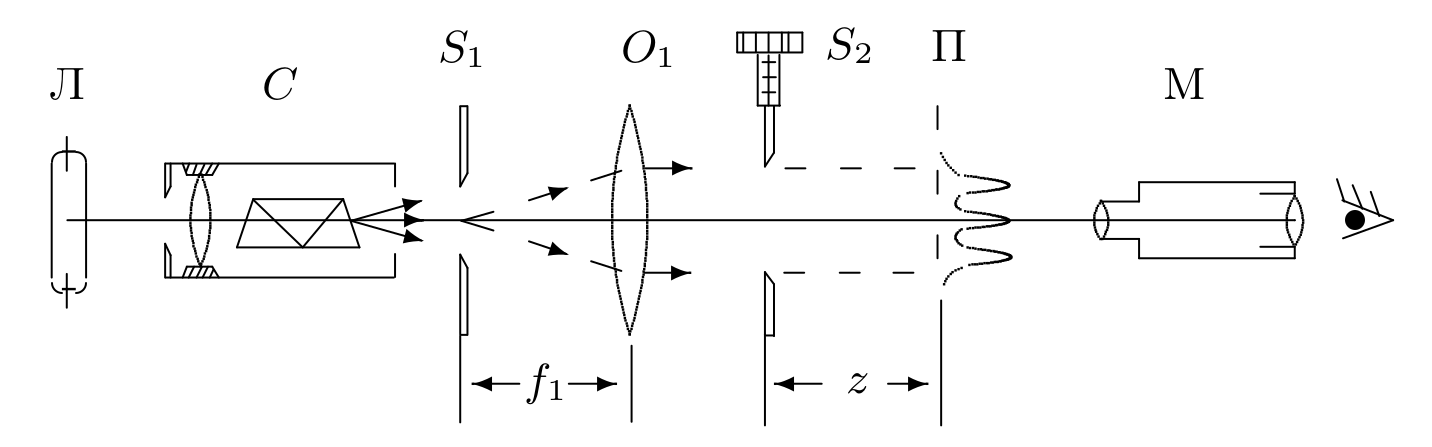
\includegraphics[width=0.9\textwidth]{../Изображения/Схема установки. Дифракция Френеля.png}
	\caption{Схема экспериментальной установки}
\end{figure}

Пучок света от ртутной лампы(Л) проходит через монохроматическую пластинку, из него выделяется световая линия средней длины $\lambda = 578 нм$. Дальше полученный пучок падает на щель(S$_1$), которая находится в фокусе собирающей линзы(O$_1$) с фокусным расстоянием 10.2см. Фронт пучка, в данный момент проходящий через щель в соответствии с принципом Гюйгенса-Френеля рассматривается как источник. Параллельный после линзы пучок падает на вторую щель(S$_2$) и испытывает на ней дифракцию, которую мы изучаем с помощью микроскопа(М), сфокусированного на некоторую плоскость наблюдения(П).\\

Схема экспериментальной установки для исследования дифракции Фраунгофера на щели приведена на рисунке:

\begin{figure}[H]
	\centering
	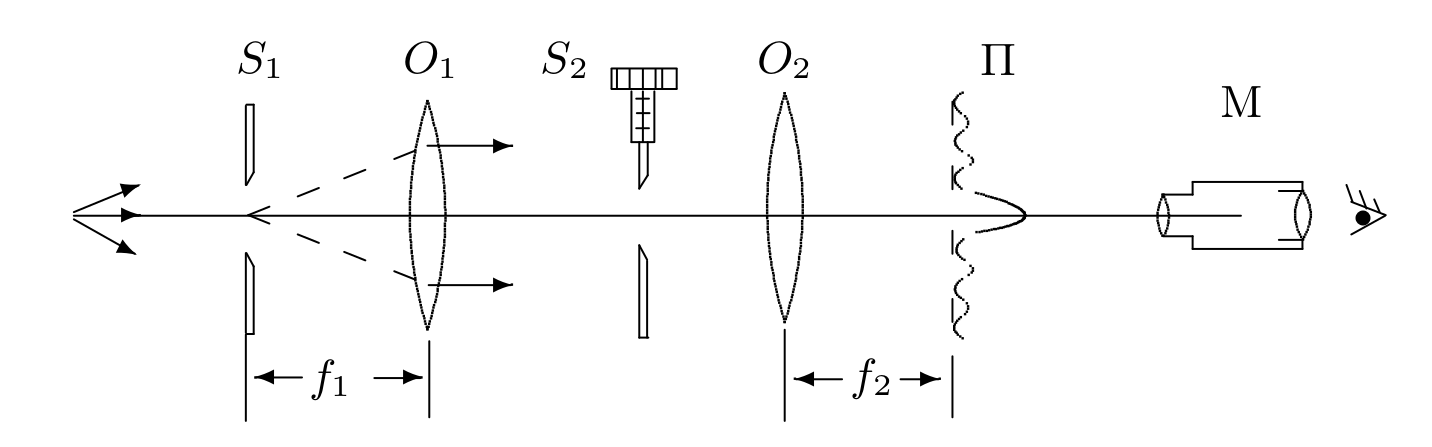
\includegraphics[width=0.9\textwidth]{../Изображения/Схема установки. Дифракция Фраунгофера.png}
	\caption{Схема экспериментальной установки}
\end{figure}

Отличие от предыдущей установки заключается в наличии второй линзы(O$_2$) с фокусным расстоянием 16см, создающей в фокальной плоскости изображение, соответствующее бесконечно удалённой плоскости наблюдения. Иначе для наблюдения дифракции Фраунгоффера пришлось бы значительно уменьшить щель(S$_2$), жертвуя освещённостью.\\

Схема экспериментальной установки для исследования дифракции Фраунгофера на двух щелях приведена на рисунке:

\begin{figure}[H]
	\centering
	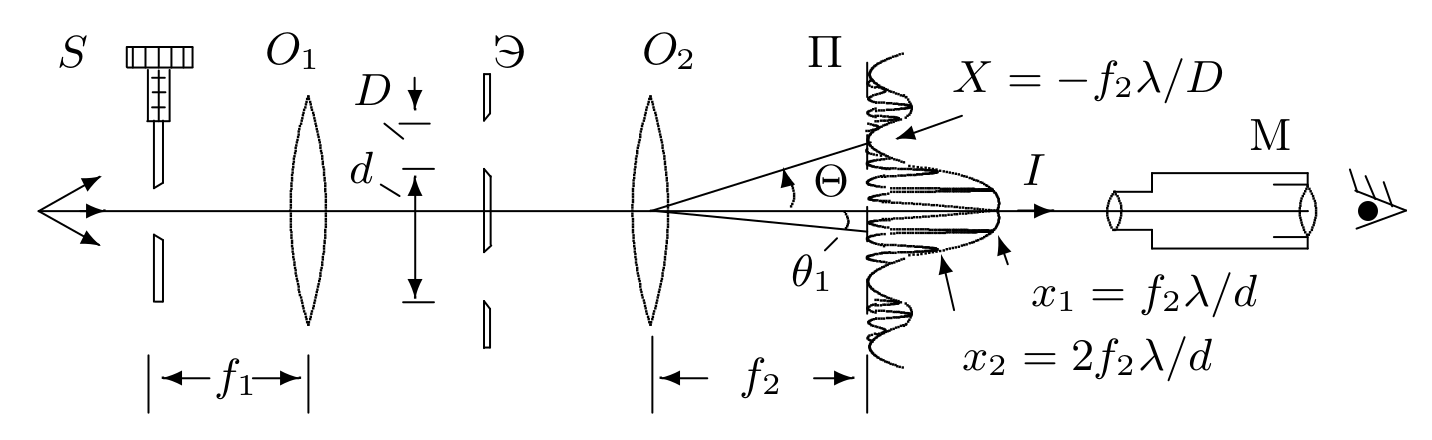
\includegraphics[width=0.9\textwidth]{../Изображения/Схема установки. Дифракция Фраунгофера, две щели.png}
	\caption{Схема экспериментальной установки}
\end{figure}

Для наблюдения дифракции Фраунгофера на двух щелях в прошлой установке вместо второй щели ставится экран(Э) с двумя щелями. Щель(S$_2$) с микрометром при этом для повышения точности ставится вместо входной щели(S$_1$). При этом на плоскости наблюдения накладываются две дифракции: с левой и правой щели.\\

Схема экспериментальной установки для исследования влияния дифракции на разрешающую способность оптического прибора приведена на рисунке:

\begin{figure}[H]
	\centering
	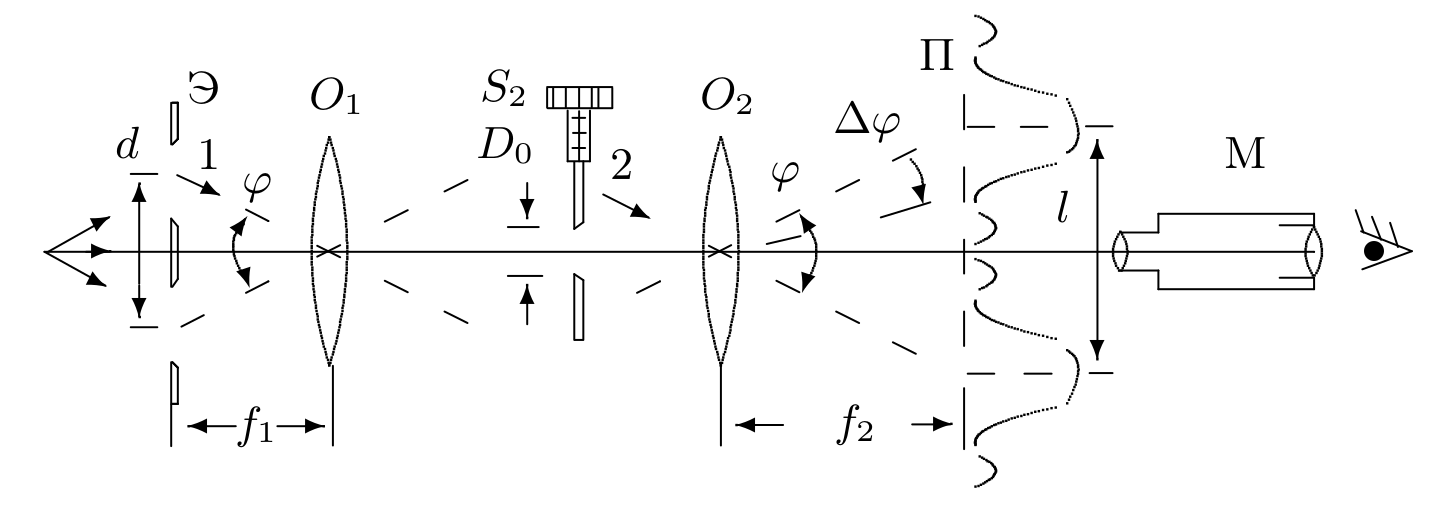
\includegraphics[width=0.9\textwidth]{../Изображения/Схема установки. Разрешающая способность.png}
	\caption{Схема экспериментальной установки}
	
Установка с двумя линзами и без второй щели создает в плоскости(П) изображение предмета, в данном случае входной щели(S$_1$). Для исследования разрещаюшей способности входная щель(S$_1$) заменяется на экран с двумя щелями(Э) (чтобы исследовать расстояние между изображениями), а между линзами ставится щель с микрометром(S$_2$).

\end{figure}

